\chapter{Addytywna synteza dźwięku}\label{chapter_additive}
Synteza addytywna pozwala na utworzenie barwy dźwięku poprzez zbudowanie pełnego widma częstotliwościowego za pomocą wybranych składowych. Słowo "addytywna" odnosi się do sumowania wielu przebiegów w jeden złożony sygnał dźwiękowy. Historycznie metoda ta jest drugą najstarszą metodą syntezy, zaraz po subtraktywnej, opisanej w rozdziale \ref{chapter_subtractive}.
Zazwyczaj synteza addytywna polega na dodawaniu sygnałów reprezentujących wiele fal sinusoidalnych o różnych częstotliwościach oraz amplitudach. Metoda ta daje użytkownikowi wiele różnorodnych możliwości. Dodawanymi składowywmi sygnału nie muszą być jedynie fale sinusoidalne.
Synteza addytywna uznawana jest za odwrotność syntezy subtraktywnej. Znajduje zastosowanie w~syntezie dźwięku oraz mowy.

W niniejszym rozdziale przedstawiono zasadę działania syntezy addytywnej. Zaprezentowano wzory matematyczne, za pomocą których można uzyskać zaprojektowane brzmienie. Przedstawiono również kilka metod implementacji tego rodzaju syntezy. Na końcu rozdziału omówiono autorski interfejs użytkownika oraz wyniki realizacji syntezy addytywnej na procesorze DSP.

\section{Zasada działania syntezy addytywnej}
Synteza addytywna jest zbliżona pod niektórymi względami do analizy częstotliwościowej Fouriera. Z tego powodu jest ona zaliczana do widmowych metod syntezy. Jej postać matematyczną można jednak przedstawić również w dziedzinie czasu. Zależnie od doboru składowych dźwięku, postać syntezy addytywnej może mieć różne reprezentacje \cite{add_defins}.
%https://ccrma.stanford.edu/~jos/sasp/Additive_Synthesis_Early_Sinusoidal.html

\subsection{Postać harmoniczna} \label{pos_harm}
Dźwięk powstały w wyniku użycia syntezy addytywnej w formie harmonicznej można zapisać za pomocą wzoru:
%https://en.wikipedia.org/wiki/Additive_synthesis#:~:text=Additive%20synthesis%20is%20a%20sound,or%20inharmonic%20partials%20or%20overtones.
\begin{equation} \label{equ:addit_time_harm}
y(t) = \sum_{k=1}^{K} a_{k}\text{sin}(2\pi kf_{0}t + \phi_{k})  \\  
\end{equation}
\begin{tabular}{ l l l l}
	gdzie: & $y(t)$ &  - & sygnał wyjściowy addytywnej syntezy dźwięku, \\
	&	$k$ & - &  numer składowej harmonicznej sygnału, \\
	&	$K$ & - &  całkowita liczba składowych harmonicznych dźwięku,\\
	&	$f_{0}$ & - &  częstotliwość pierwszej składowej harmonicznej,\\
	&	$a_{k}$ & - &  amplituda składowej harmonicznej k, \\
	&	$\phi_{k}$ & - &  faza składowej harmonicznej k. \\
\end{tabular} \\

Każda składowa dźwięku uzyskanego z takiej postaci syntezy addytywnej jest wielokrotnością częstotliwości podstawowej $f_{0}$. Wykorzystanie takiej postaci pozwala przykładowo na wygenerowanie dźwięku organów. Jest to najbardziej podstawowy rodzaj syntezy addytywnej.

%https://en.wikibooks.org/wiki/Sound_Synthesis_Theory/Additive_Synthesis <<---- SCHEMAT 

Postać harmoniczna syntezy addytywnej pozwala również na uzyskanie podstawowych przebiegów używanych w syntezie subtraktywnej. Każdy z nich można wygenerować za pomocą sumowania odpowiednich składowych harmonicznych z odpowiednimi amplitudami. Przykłady takich przebiegów w formie ciągłoczasowej przedstawiono we wzorach (\ref{equ:addit_sqr}), (\ref{equ:addit_trng}) oraz (\ref{equ:addit_sawth}).

%https://en.wikipedia.org/wiki/Square_wave
\begin{equation} \label{equ:addit_sqr}
y_{Square}(t) = \sum_{k=1}^{K} \frac{1}{2k-1} \text{sin}(2\pi (2k-1)f_{0}t), \\
\end{equation}

%https://en.wikipedia.org/wiki/Triangle_wave
\begin{equation} \label{equ:addit_trng}
y_{Triangle}(t) = \sum_{k=1}^{K} \frac{(-1)^k}{(2k-1)^2} \text{sin}(2\pi (2k-1)f_{0}t),  \\
\end{equation}

%https://en.wikipedia.org/wiki/Sawtooth_wave
\begin{equation} \label{equ:addit_sawth}
y_{Sawtooth}(t) = \sum_{k=1}^{K} \frac{(-1)^k}{k} \text{sin}(2\pi kf_{0}t). \\
\end{equation}
% O tym że na tym polegały organy Hammonda

Na rysunku \ref{rys:add_sawtooth} przedstawiono wygenerowany przebieg piłokształtny, jako przykład addytywnej syntezy dźwięku w postaci harmonicznej. Na pierwszym z wykresów przedstawiono przebieg uzyskany z dwóch składowych harmonicznych, a na kolejnym z dziesięciu. Na ostatnim wykresie widać przebieg składający się z 50 SH, który jest dobrą aproksymacją idealnego przebiegu piłokształtnego. Sygnał został wygenerowany na podstawie wzoru (\ref{equ:addit_sawth}).

\begin{figure}[H]
	\centering
	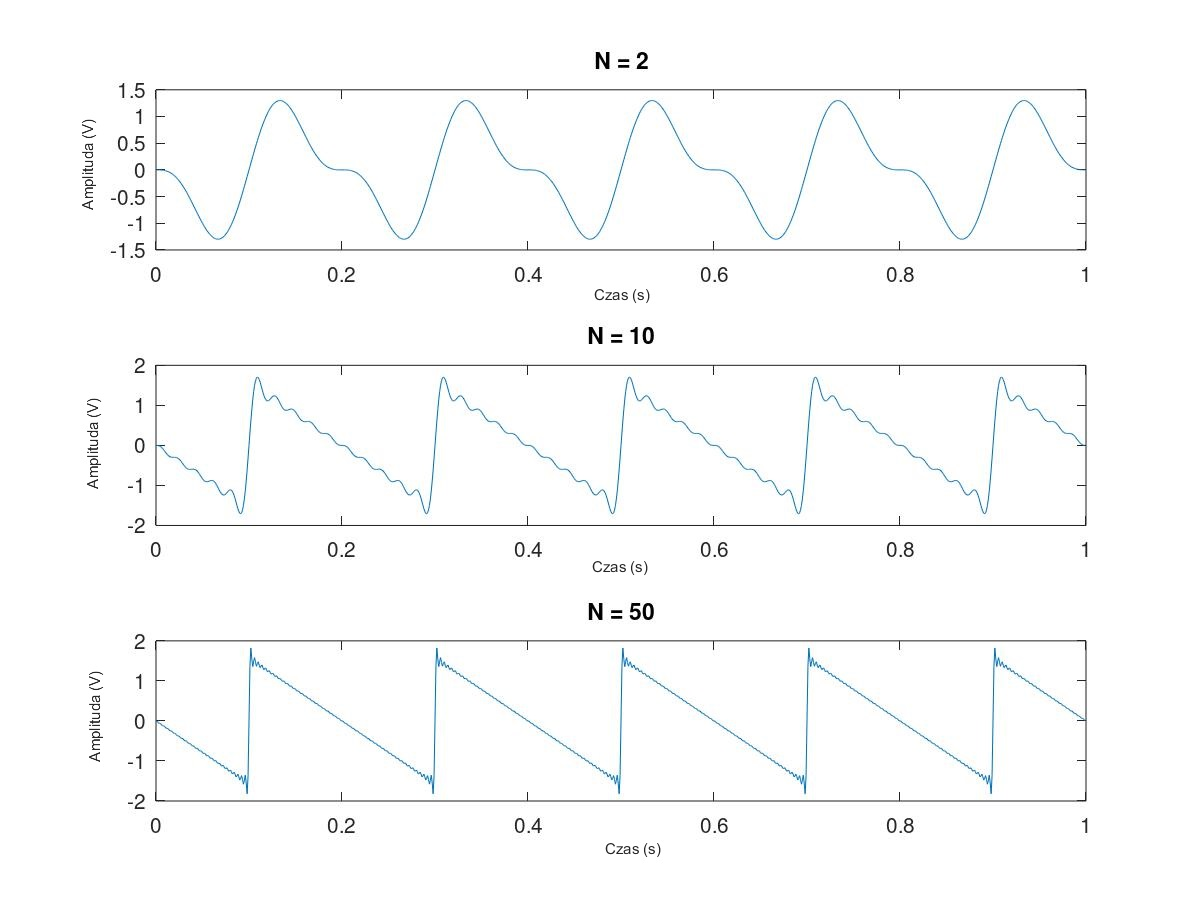
\includegraphics[width=12cm]{grafiki/add_sawtooth}
	\captionsetup{justification=centering}
	\caption{Generacja przebiegu piłokształtnego za pomocą syntezy addytywnej.}
	\label{rys:add_sawtooth}
\end{figure}

\subsection{Postać nieharmoniczna} \label{pos_nieharm}
Dobieranie składowych dźwięku w syntezie addytywnej nie musi zależeć od aktualnie wybranej częstotliwości podstawowej. Niektóre instrumenty wydają dźwięk składający się ze składowych harmonicznych oraz nieharmonicznych (czyli takich, które nie są całkowitą wielokrotnością pewnej częstotliwości $f_{0}$). Zsyntezowany dźwięk w takiej postaci można opisać wzorem:
\begin{equation} \label{equ:addit_time_nieharm}
y(t) = \sum_{k=1}^{K} a_{k}\text{sin}(2\pi f_{k}t + \phi_{k})  \\  
\end{equation}
\begin{tabular}{ l l l l}
	gdzie: 	&	$f_{k}$ & - &  częstotliwość składowej sygnału k. \\
\end{tabular} \\

Postać (\ref{equ:addit_time_nieharm}) można traktować jako uogólnioną formę wzoru (\ref{equ:addit_time_harm}). Częstotliwość $f_k$ to taka, która zazwyczaj nie jest całkowitą wielokrotnością częstotliwości $f_0$. Dźwięk opisany powyższym wzorem jest generowany przez instrumenty takie jak dzwony lub perkusjonalia.

\subsection{Składowe zmienne w czasie}
%https://books.google.pl/books/about/The_Computer_Music_Tutorial.html?id=nZ-TetwzVcIC&printsec=frontcover&source=kp_read_button&redir_esc=y#v=onepage&q&f=false  , strona 140
Wzory matematyczne (\ref{equ:addit_time_harm}) i (\ref{equ:addit_time_nieharm}) pozwalają na uzyskanie jedynie stanu ustalonego zsyntezowanego brzmienia. Powtarzany jest jeden okres sygnału, co daje wrażenie słuchaczowi stałości parametrów powtarzanego dźwięku.

Składowe sygnału audio mogą jednak zmieniać się w czasie \cite{add_time_varying}. Zmiany te mogą dotyczyć ich amplitudy, jak i częstotliwości.
Taką postać syntezy addytywnej zapisuje się jako:
\begin{equation} \label{equ:addit_time_zmienne}
y(t) = \sum_{k=1}^{K} a_{k}(t)\text{sin}(2\pi f_{k}(t)t + \phi_{k})  \\  
\end{equation}
\begin{tabular}{ l l l l}
	gdzie: & $a_{k}(t)$ &  - & zmienna w czasie amplituda składowej k, \\
	&	$f_{k}(t)$ & - &  zmienna w czasie częstotliwość składowej k. \\
\end{tabular} \\

Realizacja brzmienia na podstawie wzoru (\ref{equ:addit_time_zmienne}) może być rozumiana jako zmiana parametrów instrumentu w trakcie generowania przez niego dźwięku.

\subsection{Szum w syntezie addytywnej}
%https://ccrma.stanford.edu/~jos/sasp/S_N_Synthesis.html
Tworzenie dźwięku zsyntezowanego metodą addytywną za pomocą wzorów przedstawionych powyżej jest deterministyczne. Do takiego sygnału może zostać dodana część stochastyczna. Uzyskuje się to przez wykorzystanie szumu białego, którego widmo kształtowane jest za pomocą filtru FIR o zmiennych w czasie parametrach \cite{add_szum}. Takie działanie zostało zaprezentowane we wzorze (\ref{equ:addit_szum}).

\begin{equation} \label{equ:addit_szum}
B(\omega) = F(\omega, t)e^{j\phi(\omega_{k})} \\  
\end{equation}
% Wprowadzic (t)
\begin{tabular}{ l l l l}
	gdzie: & $\phi(\omega_{k})$ &  - & faza losowa o rozkładzie równomiernym od -$\pi$ do $\pi$, \\
	& $F(\omega, t)$ &  - & obwiednia widmowa filtra FIR o zmiennych parametrach w czasie, \\
	% TU DOPISAC B(w) wyjasnienie
	&	$B(\omega)$ & - & widmo powstałej części stochastycznej. \\
\end{tabular} \\

%Synteza części stochastycznej polega na przetwarzaniu białego szumu (bazującego na losowej fazie) przez filtr FIR.
% Zajrzec do wykladu Niedzwieckiego
Po wykonaniu zależności (\ref{equ:addit_szum}), część stochastyczna zostaje przetransformowana do dziedziny czasu. Ostatnim krokiem jest zsumowanie ze sobą obu części.

Dodanie szumu do sygnału deterministycznego w syntezie addytywnej pozwala na uzyskanie dźwięków na przykład instrumentów dętych. Część stochastyczna sygnału sprawia wrażenie pobudzenia rzeczywistego stroika instrumentu strumieniem powietrza.

% Mozna jeszcze to użyć:
%https://ccrma.stanford.edu/~jos/sasp/Sines_Noise_Analysis.html

\section{Metody implementacji syntezy addytywnej}
Istnieją różne metody implementacji addytywnej syntezy dźwięku \cite{add_imp_meth}. Oznacza to, iż ten sam dźwięk może zostać uzyskany różnymi sposobami. Popularne metody realizacji syntezy addytywnej to:
\begin{itemize}
	\item bank oscylatorów,
	\item synteza wavetable,
	\item synteza IFFT.
	% https://ieeexplore.ieee.org/document/4412805
\end{itemize}
W niniejszym podrozdziale przedstawiono ograniczenia syntezy addytywnej oraz omówiono wymienione wyżej metody implementacji.

\subsection{Ograniczenia syntezy addytywnej} \label{addit_ograniczenia}
%https://en.wikipedia.org/wiki/Additive_synthesis#History
Synteza addytywna w instrumentach klawiszowych jest używana między innymi do generacji dźwięku organów, których barwa upraszczana jest zazwyczaj do kilku SH. W przypadku próby uzyskania dźwięku o większej liczbie składowych harmonicznych, złożoność obliczeniowa metody wzrasta \cite{add_ograniczenia}.
%https://ccrma.stanford.edu/~jos/pasp/Additive_Synthesis.html
Przykładowo, dla uzyskania pojedynczego dźwięku fortepianu w jakości CD-Audio,
%https://en.wikipedia.org/wiki/Compact_Disc_Digital_Audio
wymagane byłoby obliczenie około 400 fal sinusoidalnych na każdą próbkę zsyntezowanego dźwięku. Oznacza to, iż dla polifonicznej klawiatury takiego pianina mogłyby być to tysiące składowych przypadających na jedną próbkę. Z uwagi na zbyt dużą złożoność obliczeniową. obecne ograniczenia sprzętowe nie umożliwiają realizacji w czasie rzeczywistym tak skomplikowanych brzmień, za pomocą syntezy addytywnej. Powstrzymują one szybki rozwój tej metody.

\subsection{Bank oscylatorów}
%analogowe hammondy i zwykłe, ale ze są wolne
Synteza za pomocą banku oscylatorów jest najstarszą metodą implementacji addytywnej syntezy dźwięku. Opiera się ona bezpośrednio na równaniu (\ref{equ:addit_time_harm}).
Ta metoda implementacji realizowana była nawet na instrumentach analogowych. Instrumenty takie jak organy Hammonda miały kilka wirujących dysków (koła tonacyjne) posiadających w wielu miejscach nacięcia o specyficznych kształtach. Obracające tarcze powodowały zmiany w polu magnetycznym, co generowało małe napięcia w zwojnicy. Dzięki temu uzyskiwano prąd elektryczny o charakterystyce zawierającej pewne składowe harmoniczne tonu podstawowego.
% Przez te tarcze oswietlana byla fotokomorka
\begin{figure}[H]
	\centering
	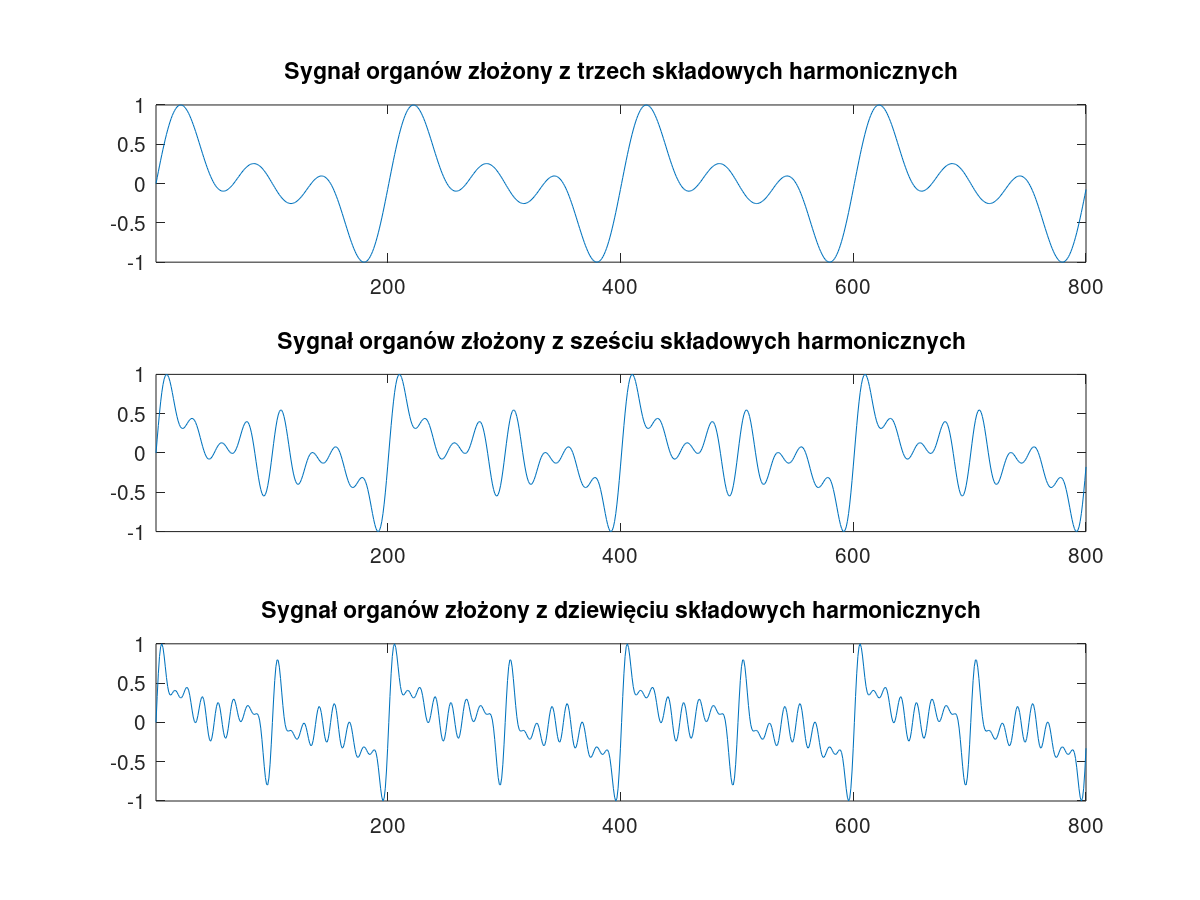
\includegraphics[width=15cm]{grafiki/add_hammond_matlab}
	\captionsetup{justification=centering}
	\caption{Barwa dźwięku organów Hammonda dla różnych ilości składowych harmonicznych.}
	\label{rys:add_hammond_matlab}
\end{figure}

Implementacja na procesorach DSP, odpowiadająca wirującym dyskom, opiera się na sumowaniu wielu funkcji sin() posiadających różne częstotliwości i amplitudy. Każda taka funkcja generuje jedną składową harmoniczną syntezowanego dźwięku. Wszystkie razem traktowane są jako bank oscylatorów. Problem realizacji skomplikowanego brzmienia takim sposobem został przedstawiony w punkcie \ref{addit_ograniczenia}.

Na rysunku \ref{rys:add_hammond_matlab} przedstawiono wygenerowaną barwę organów Hammonda dla trzech różnych ustawień amplitud składowych harmonicznych. Najbardziej zauważalna różnica występuje między pierwszym i ostatnim wykresem. 
Sumowanie jedynie trzech SH pozwala uzyskać dźwięk prosty, podobny do brzmienia organów piszczałkowych. Natomiast dodanie dziewięciu składowych harmonicznych bardzo wzbogaca charakter zsyntezowanego brzmienia, które upodabnia się do dźwięków organów stosowanych w muzyce rockowej.

\subsection{Synteza wavetable} \label{add_wavetable}
%opisac tą która została zaimplementowana
Synteza wavetable (nazywana również syntezą tablicową) polega na zapisaniu jednego okresu fali dźwiękowej do tablicy typu lookup, zdefiniowanej w programie komputerowym \cite{add_wavetab_synt}. W każdej kolejnej chwili czasu działania programu, odczytywany jest odpowiedni element tablicy. Sygnał zapisany w tablicy powinien zostać kilkukrotnie nadpróbkowany (ang. over-sampled), aby móc odczytać go dla fal o niskich częstotliwościach. 
Odtwarzanie wszystkich próbek w opisanej tablicy pozwala uzyskać najniższą częstotliwość fali $f_0$. Wybieranie co drugiej próbki powoduje generowanie częstototliwości 2$f_0$, co trzeciej 3$f_0$ i tak dalej.
% Generowanie dźwięków o okreslonej czestotliwosci polega na wybieraniu 

W syntezie addytywnej użycie takiej metody implementacji może znacznie przyspieszyć generowanie kolejnych próbek składowych sygnału. Do tablicy zapisuje się jeden przebieg sinusoidalny. Odczyt jednego indeksu zabiera mniej czasu pracy procesora niż wygenerowanie próbki za pomocą funkcji sin(). Działanie takiej metody jest podobne do banku oscylatorów, ze względu na działanie w dziedzinie czasu. Różnica polega na tym, że tablicę w syntezie wavetable można traktować jako jeden oscylator, z którego należy jedynie odczytać wartości tj. znaleźć odpowiedni indeks tablicy (nie jest konieczne obliczanie na nowo próbki dla każdej składowej dźwięku, w~każdej chwili czasu).
%https://en.wikipedia.org/wiki/Lookup_table

\subsection{Synteza IFFT}
%Rysunki z matlaba
W 1990 roku P. Depalle oraz X. Rodet \cite{add_ifft_orig} przedstawili przełomową metodę implementacji syntezy addytywnej. W zaproponowanym przez nich rozwiązaniu, obliczanie składowych dźwięku nie opiera się na zestawie oscylatorów, lecz na algorytmie IFFT (ang. Inverse Fast Fourier Transform) stosowanym dla krótkookresowej analizy częstotliwościowej (STS, ang. short term spectrum) \cite{add_ifft_method}. Wyniki ich pracy dowiodły, iż w stosunku do metody banku oscylatorów udało się zmniejszyć koszt obliczeń syntezy addytywnej piętnastokrotnie (w omawianym przez autorów przypadku, gdzie obliczano 9 istotnych punktów widma w 256 próbkowym STS).

% POPRAWIĆ - DOCZYTAĆ

% polega na tym ze posuwamy sie po danych i wycinamy jakis fragment danych, a potem hanning jest i mamy W[]

% Oznaczając przez W transformatę Fouriera funckji okienkującej sygnał w[n],
% Dodanie skladowej do STS moze byc zapisane zależnoscią.

Konstrukcja pojedynczej ramki STS została przedstawiona poniżej. Niech $f_{j}$, $a_{j}$ oraz $\phi_{j}$ będą wartościami częstotliwości, amplitudy i fazy ramki czasowej składowej $j$ pożądanego sygnału $s[n]$. $W[k]$ niech będzie Transformatą Fouriera okna Hanninga $w[n]$. Widmo generowanego sygnału tworzone jest z pojedynczych prążków. W niektórych sytuacjach składową należy wyrazić za pomocą kilku prążków widma (centrowanie widma wokół częstotliwości prążka). Dodanie pojedynczej składowej do STS może zostać zapisane zależnością:

\begin{equation} \label{equ:addit_IFFT}
S[k] = a_{j}e^{i\phi_{j}}W[f_{j} - k] \\  
\end{equation}
\begin{tabular}{ l l l l}
	gdzie: & $S[k]$ &  - & STS syntezowanego sygnału, \\
	& $W[f_{j} - k]$ &  - & przesunięte w częstotliwości widmo okna Hanninga, \\
	& $a_{j}e^{i\phi_{j}}$ & - & zespolona amplituda. \\
\end{tabular} \\

Wzór (\ref{equ:addit_IFFT}) oznacza, iż widmo dyskretne $W[f_{j} - k]$ zostanie wycentrowane na prążku częstotliwości $f_{j}$ oraz przemnożone przez amplitudę $a_{j}e^{i\phi_{j}}$. Po takim działaniu w dziedzinie częstotliwości, widmo dyskretne $S[k]$ jest poddane algorytmowi IFFT, którego rezultatem jest sygnał $s[n]$, który odpowiada przetworzonemu fragmentowi $w[n]$. Kolejne okna czasowe zakładkowane są metodą overlap-add. Końcowo otrzymuje się pełen sygnał wygenerowanego dźwięku za pomocą syntezy IFFT.

Dodanie szumu do sygnału jest również bardziej efektywne obliczeniowo w przypadku stosowania opisywanej metody implementacji syntezy addytywnej. Szum biały może zostać dodany już na etapie tworzenia STS, a następnie poddany algorytmowi IFFT. Ostatecznie uzyskiwane jest okno sygnału zawierającego część deterministyczną, jak i stochastyczną.

\section{Interfejs użytkownika}
W autorskim projekcie, w ramach realizacji instrumentu klawiszowego z syntezą addytywną, zaimplementowano program generujący dźwięk organów Hammonda. 
%https://www.soundonsound.com/techniques/synthesizing-tonewheel-organs-part-1
Laurens Hammond, twórca tychże organów, zaprojektował je tak, aby użytkownik miał możliwość doboru amplitudy dziewięciu składowych harmonicznych generowanego dźwięku \cite{add_hammond_soundonsound}. Każda z nich była regulowana suwakiem na 8 możliwych poziomów. Suwaki oznaczały kolejne wartości amplitudy pierwszej, drugiej, trzeciej, czwartej, szóstej, ósmej, dziesiątej, dwunastej oraz szesnastej składowej harmonicznej dźwięku. Przykładowe różnice w generowanej barwie organów przedstawione zostały na rysunku \ref{rys:add_hammond_matlab}.

% Wyjasnic numery harmonicznych na rysunku
\begin{figure}[H]
	\centering
	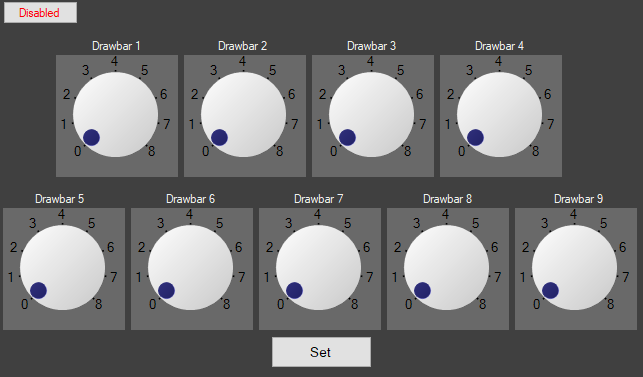
\includegraphics[width=15cm]{grafiki/add_interface}
	\captionsetup{justification=centering}
	\caption{Interfejs użytkownika modułu syntezy addytywnej. Numery gałek odpowiadają kolejnym suwakom w organach Hammonda.}
	\label{rys:add_interface}
\end{figure}

Interfejs programu opiera się na oryginalnym instrumencie Laurensa Hammonda. Umożliwia on użytkownikowi regulację dziewięciu SH za pomocą gałek przedstawionych na rysunku \ref{rys:add_interface}. Można zauważyć, iż gałki posiadają również 8 poziomów wartości, które odpowiadają wartościom amplitud składowych harmonicznych. Po ustawieniu pożądanej barwy, użytkownik musi kliknąć na panelu w przycisk "Set", aby parametry syntezy addytywnej zostały wysłane do procesora DSP.

Gałki panelu zostały zrealizowane za pomocą obiektów klasy KnobControl. Naciśnięcie przycisku "Set" wywołuje funkcję, która odczytuje wartość elementu panelu syntezy addytywnej w formie tablicy bajtów. Następnie program wysyła odpowiedni identyfikator gałki do procesora DSP, a~po nim jej wartość odczytaną z tablicy.

\section{Realizacja organów na procesorze DSP}
Pierwszą próbą implementacji organów Hammonda w autorskim programie dla procesora DSP, było wykorzystanie metody banku oscylatorów. Rezultaty były jednak niezadowalające. Wywołanie funkcji sin() dziwięciokrotnie dla jednej próbki sygnału, oznaczało, iż w podejściu polifonicznym mogła ona zostać wywołana nawet dziewiędziesiąt razy (odpowiada to sytuacji naciśnięcia dziesięciu klawiszy na klawiaturze MIDI).
Pomimo zastosowanego mechanizmu zakładkowania, w generowanym dźwięku pojawiały się niepożądane artefakty świadczące o zbyt dużej złożoności obliczeniowej zaimplementowanego algorytmu. Należało zmienić podejście do implementacji syntezy addytywnej.

Ostatecznie w autorskim programie komputerowym na procesor DSP wykorzystano metodę implementacji z użyciem tablicy wavetable, która została omówiona w punkcie \ref{add_wavetable}. W niniejszym podrozdziale został przedstawiony sposób realizacji programu umożliwiającego syntezę dźwięku organów Hammonda oraz rezultaty takiej syntezy z wykorzystaniem układu TMS320C6727.

\subsection{Opis implementacji}
Zdefiniowana tablica lookup o nazwie sinLut[.] zawiera jeden okres fali sinusoidalnej. Wypełniona zostaje danymi na etapie inicjalizacji programu na procesorze DSP. Każda wartość tablicy zostaje odczytana za pomocą funkcji mySin(), która jako argumenty przyjmuje częstotliwość pożądanej fali sinusoidalnej oraz jej przesunięcie w fazie.
\begin{equation} \label{equ:addit_sinLut}
\text{samp} = \text{sinLut}[(kf\frac{N}{F_s})\mod{N}] \\  
\end{equation}
\begin{tabular}{ l l l l}
	gdzie: & \text{samp} &  - & wartość próbki odczytywanej z tablicy sinLut[.], \\
	& $k$ &  - & licznik odczytu odpowiedniej próbki z tablicy sinLut[.], \\
	& $f$ & - & częstotliwość sinusoidy, \\
	& $N$ & - & długość tablicy sinLut[.], \\
	& $F_s$ & - & częstotliwość próbkowania DAC. \\
\end{tabular} \\

Funkcja mySin() zwraca element z tablicy na podstawie wzoru (\ref{equ:addit_sinLut}). Do wygenerowania jednej próbki organów Hammonda sumowane jest 9 tak odczytanych wartości sinLut[.] (odpowiadających składowym harmonicznym). Każda próbka zsyntezowanego dźwięku ulega wymnożeniu z~obecną wartością amplitudy ADSR. Opisana czynność wykonywana jest tyle razy, ile elementów posiada jeden blok generowanego sygnału.

Procesor DSP otrzymuje z interfejsu użytkownika nastawy gałek regulatorów syntezy addytywnej za pomocą funkcji obsługi przerwania UART. Parametry te są zapisywane do tablicy add\_knobAmp[.]. Następnie są używane do syntezy dźwięku organów.

\subsection{Wyniki}
Wykorzystana metoda implementacji za pomocą tablicy wavetable umożliwiła jednoczesne wykorzystanie kilkunastu klawiszy instrumentu, bez pojawienia się niepożądanych artefaktów w~dźwięku. Zmiany amplitud poszczególnych składowych harmonicznych wpływają na generowane brzmienie w bardzo wyraźny sposób.

\begin{figure}[H]
	\centering
	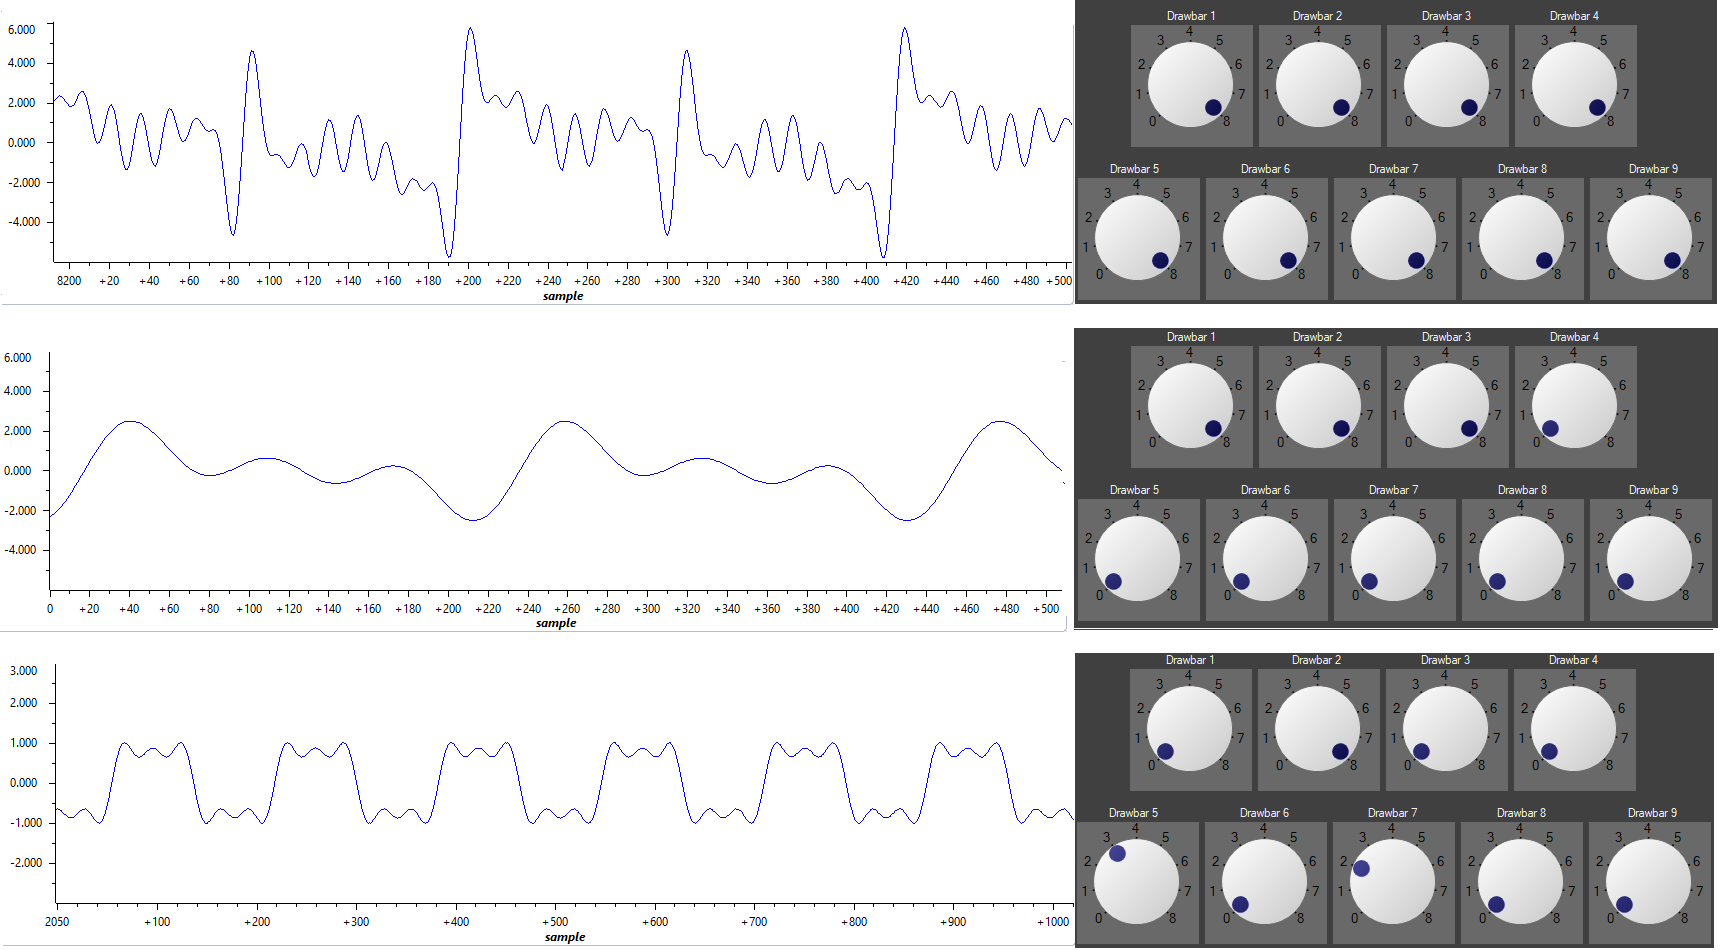
\includegraphics[width=15cm]{grafiki/add_hammond_dsp}
	\captionsetup{justification=centering}
	\caption{Wizualizacja sygnału dźwiękowego organów Hammonda z procesora DSP dla różnych nastaw gałek.}
	\label{rys:add_hammond_dsp}
\end{figure}

Na rysunku \ref{rys:add_hammond_dsp} przedstawiono wizualizację sygnału organów dla różnych ustawień gałek regulatorów interfejsu użytkownika. Na wykresie pierwszym od góry wszystkie SH mają maksymalną amplitudę (konfiguracja "8888 88888"). Tak wygenerowany dźwięk bardzo przypomina brzmienie katedralnych organów piszczałkowych. Na kolejnym wykresie przedstawiono sygnał utworzony przy konfiguracji gałek na wartościach "8880 00000". Brzmienie dźwięku przy takim ustawieniu jest dużo bardziej delikatne niż w pierwszej konfiguracji. Na najniższym wykresie ustawienie amplitud to "0800 30200". Można zauważyć, iż wizualnie bardzo przypomina przebieg prostokątny. Brzmienie tak wygenerowanego dźwięku również jest zbliżone do dźwięku przebiegu prostokątnego.

Przedstawione barwy organów mogą być jeszcze bardziej urozmaicone po dodaniu takich efektów jak Chorus lub Vibrato. Dla uzyskania pełni brzmienia organów, często stosuje się również efekt pogłosu (ang. reverb).